\documentclass[notheorems,final]{beamer}
\mode<presentation>{
  \usetheme{cuposter}
}
\usepackage[english]{babel}
\usepackage[latin1]{inputenc}
\usepackage{amsmath,amsthm, amssymb, latexsym}
\usefonttheme[onlymath]{serif}
\boldmath
\usepackage[orientation=landscape,size=a0,scale=1.4,debug]{beamerposter}
\usepackage{algorithm,algorithmic}
\title{Mixing Time Estimation in Reversible Markov Chains from a Single Sample Path}
\author{%
  Daniel Hsu$^\dag$,
  Aryeh Kontorovich$^\sharp$,
  Csaba Szepesv\'ari$^\star$%
}
\institute{%
  $^\dag$Columbia University,
  $^\sharp$Ben-Gurion University,
  $^\star$University of Alberta%
}

\newcommand{\compresslist}{%
  \setlength{\itemsep}{1pt}%
  \setlength{\parskip}{0pt}%
  \setlength{\parsep}{0pt}%
  \setlength{\leftmargin}{0.7cm}%
}

\newlength{\columnheight}
\setlength{\columnheight}{70cm}

%!TEX root =  matrix-est.tex
%\usepackage{etex} % handle MANY packages

% comment this out for the final version, or add the final option:
%\usepackage[notcite,notref]{showkeys}


\usepackage{amsmath,amsbsy,amsfonts,amssymb,amsthm,color,dsfont,mleftright,nccmath}
\usepackage{url}
\usepackage{dsfont} % double stroke font

%%%%%%%%%%%%%%%%%%%%%%%%%%%%%%%%
% PACKAGES
%%%%%%%%%%%%%%%%%%%%%%%%%%%%%%%%
\setlength{\marginparwidth}{25mm}
%\usepackage[textsize=tiny]{todonotes}
\usepackage[disable]{todonotes}
\newcommand{\todoc}[2][]{\todo[color=red!20!white,#1]{Cs: #2}}
\newcommand{\todod}[2][]{\todo[color=blue!20!white,#1]{D: #2}}
\newcommand{\todoa}[2][]{\todo[color=green!20!white,#1]{A: #2}}

\newcommand{\hide}[1]{}

% turn off previously defined macros as we want to use ntheorem (jmlr foolishly defines these)
\if0
\let\proof\relax
\let\endproof\relax
\let\theorem\relax
\let\endtheorem\relax
\let\proposition\relax
\let\endproposition\relax
\let\lemma\relax
\let\endlemma\relax
\let\corollary\relax
\let\endcorollary\relax
\let\example\relax
\let\endexample\relax
\let\remark\relax
\let\endremark\relax
\let\definition\relax
\let\enddefinition\relax
\fi
%\usepackage[amsmath,standard,thmmarks]{ntheorem} % ntheorem makes cleveref work properly 
\newtheorem{lemma}{Lemma}
\newtheorem{claim}{Claim}
\newtheorem{proposition}{Proposition}
\newtheorem{theorem}{Theorem}
\newtheorem{corollary}{Corollary}

\usepackage{latexsym}
%\usepackage{times}
\usepackage{mathtools}
\usepackage{enumerate}
\usepackage[ruled]{algorithm}
\usepackage{algorithmic}
\usepackage{hyperref}
\hypersetup{
    bookmarks=true,         % show bookmarks bar?
    unicode=false,          % non-Latin characters in Acrobat's bookmarks
    pdftoolbar=true,        % show Acrobat's toolbar?
    pdfmenubar=true,        % show Acrobat's menu?
    pdffitwindow=false,     % window fit to page when opened
    pdfstartview={FitH},    % fits the width of the page to the window
    pdftitle={My title},    % title
    pdfauthor={Author},     % author
    pdfsubject={Subject},   % subject of the document
    pdfcreator={Creator},   % creator of the document
    pdfproducer={Producer}, % producer of the document
    pdfkeywords={keyword1} {key2} {key3}, % list of keywords
    pdfnewwindow=true,      % links in new window
    colorlinks=true,       % false: boxed links; true: colored links
    linkcolor=red,          % color of internal links (change box color with linkbordercolor)
    citecolor=blue,        % color of links to bibliography
    filecolor=magenta,      % color of file links
    urlcolor=black          % color of external links
}
%\usepackage[standard]{ntheorem}
%\usepackage{times}
\usepackage[numbers,sort&compress]{natbib}
\usepackage{enumitem}
\usepackage{bibunits}


%\setlist{nolistsep}

%%%%%%%%%%%%%%%%%%%%%%%%%%%%%%%%
% THEOREMS
%%%%%%%%%%%%%%%%%%%%%%%%%%%%%%%%
\if0
\newtheorem{lemma}{Lemma}
\newtheorem{claim}{Claim}
\newtheorem{proposition}{Proposition}
\newtheorem{theorem}{Theorem}
\newtheorem{corollary}{Corollary}
\theoremstyle{remark}
\newtheorem{remark}{Remark}
\theoremstyle{definition}
\newtheorem{definition}{Definition}
\newtheorem{condition}{Condition}
\newtheorem{example}{Example}
\newtheorem{problem}{Problem}
\fi
\usepackage[capitalize]{cleveref}
\usepackage{fullpage}

%%%%%%%%%%%%%%%%%%%%%%%%%%%%%%%%
% MACROS
%%%%%%%%%%%%%%%%%%%%%%%%%%%%%%%%

\def\ddefloop#1{\ifx\ddefloop#1\else\ddef{#1}\expandafter\ddefloop\fi}

% \bA, \bB, ...
\def\ddef#1{\expandafter\def\csname b#1\endcsname{\ensuremath{\mathbf{#1}}}}
\ddefloop ABCDEFGHIJKLMNOPQRSTUVWXYZ\ddefloop

% \bbA, \bbB, ...
\def\ddef#1{\expandafter\def\csname bb#1\endcsname{\ensuremath{\mathbb{#1}}}}
\ddefloop ABCDEFGHIJKLMNOPQRSTUVWXYZ\ddefloop

% \cA, \cB, ...
\def\ddef#1{\expandafter\def\csname c#1\endcsname{\ensuremath{\mathcal{#1}}}}
\ddefloop ABCDEFGHIJKLMNOPQRSTUVWXYZ\ddefloop

% \vA, \vB, ..., \va, \vb, ...
\def\ddef#1{\expandafter\def\csname v#1\endcsname{\ensuremath{\boldsymbol{#1}}}}
\ddefloop ABCDEFGHIJKLMNOPQRSTUVWXYZabcdefghijklmnopqrstuvwxyz\ddefloop

% \valpha, \vbeta, ...,  \vGamma, \vDelta, ...,
\def\ddef#1{\expandafter\def\csname v#1\endcsname{\ensuremath{\boldsymbol{\csname #1\endcsname}}}}
\ddefloop {alpha}{beta}{gamma}{delta}{epsilon}{varepsilon}{zeta}{eta}{theta}{vartheta}{iota}{kappa}{lambda}{mu}{nu}{xi}{pi}{varpi}{rho}{varrho}{sigma}{varsigma}{tau}{upsilon}{phi}{varphi}{chi}{psi}{omega}{Gamma}{Delta}{Theta}{Lambda}{Xi}{Pi}{Sigma}{varSigma}{Upsilon}{Phi}{Psi}{Omega}\ddefloop

\newcommand\Sig{\ensuremath{\varSigma}}
\newcommand\veps{\ensuremath{\varepsilon}}
\newcommand\eps{\ensuremath{\epsilon}}

\renewcommand\t{{\ensuremath{\scriptscriptstyle{\top}}}}

\DeclareMathOperator{\tr}{tr}
\DeclareMathOperator{\diag}{diag}
\DeclareMathOperator{\Diag}{Diag}
\DeclareMathOperator{\rank}{rank}
\DeclareMathOperator{\sign}{sign}
\DeclareMathOperator{\supp}{supp}
\DeclareMathOperator{\vol}{vol}

\DeclareMathOperator{\var}{var}
\DeclareMathOperator{\Var}{Var}

\DeclareMathOperator{\Bd}{bd}
\DeclareMathOperator{\Cl}{cl}
\DeclareMathOperator{\Conv}{conv}
\DeclareMathOperator{\Int}{int}
\DeclareMathOperator{\Null}{ker}
\DeclareMathOperator{\Span}{span}
\DeclareMathOperator{\Range}{ran}

\DeclareMathOperator*{\argmin}{arg\,min}
\DeclareMathOperator*{\argmax}{arg\,max}

\newcommand\wt{\ensuremath{\widetilde}}
\newcommand\wh{\ensuremath{\widehat}}
\renewcommand\v{\ensuremath{\boldsymbol}}

\newcommand\comment[1]{{\color{blue}\{\textbf{Comment}: #1\}}}

\newcommand\parens[1]{(#1)}
\newcommand\norm[1]{\|#1\|}
\newcommand\braces[1]{\{#1\}}
\newcommand\brackets[1]{[#1]}
\newcommand\ceil[1]{\lceil#1\rceil}
\newcommand\abs[1]{|#1|}
\newcommand\ind[1]{\ensuremath{\mathds{1}\{#1\}}}
\newcommand\dotp[1]{\langle #1 \rangle}

\newcommand\Parens[1]{\left(#1\right)}
\newcommand\Norm[1]{\left\|#1\right\|}
\newcommand\Braces[1]{\left\{#1\right\}}
\newcommand\Brackets[1]{\left[#1\right]}
\newcommand\Ceil[1]{\left\lceil#1\right\rceil}
\newcommand\Floor[1]{\left\lfloor#1\right\rfloor}
\newcommand\Abs[1]{\left|#1\right|}
\newcommand\Ind[1]{\ensuremath{\mathds{1}\left\{#1\right\}}}
\newcommand\Dotp[1]{\left\langle #1 \right\rangle}

\newcommand\pimin{\ensuremath{\pi_{\star}}}
\newcommand\gap{\ensuremath{\gamma_{\star}}}
\newcommand\slem{\ensuremath{\lambda_{\star}}}

\newcommand\hatpimin{\ensuremath{\hat\pi_{\star}}}
\newcommand\hatgap{\ensuremath{\hat\gamma_{\star}}}

\newcommand\Geom{\ensuremath{\operatorname{Geom}}}
\newcommand\Sym{\ensuremath{\operatorname{Sym}}}
\newcommand\errm{\ensuremath{\v{\cE}_{\vM}}}
\newcommand\errp{\ensuremath{\v{\cE}_{\vpi}}}
\newcommand\errP{\ensuremath{\v{\cE}_{\vP}}}
\newcommand\errpil{\ensuremath{\v{\cE}_{\vpi,1}}}
\newcommand\errpir{\ensuremath{\v{\cE}_{\vpi,2}}}
\newcommand\tv{\ensuremath{\operatorname{tv}}}
\newcommand\tmix{\ensuremath{t_{\operatorname{mix}}}}
\newcommand\trelax{\ensuremath{t_{\operatorname{relax}}}}
\newcommand\avg{\ensuremath{\operatorname{avg}}}
\newcommand{\iset}[1]{[#1]}
\newcommand{\opencloseint}[1]{\ensuremath{(#1]}}

\newcommand{\Dvpi}{\Diag(\vpi)}
\newcommand{\Dvpit}{\Diag(\vpi^{(t)})}

\newcommand{\EE}[1]{\bbE\left(#1\right)}

\newcommand\giAh{\ensuremath{\widehat{\boldsymbol{A}}^{\raisebox{-2.9pt}{$\scriptstyle\#$}}}}
\newcommand\giA{\ensuremath{\boldsymbol{A}^{\raisebox{-0pt}{$\scriptstyle\#$}}}}
\newcommand{\defeq}{:=}

\newcommand\emptail{\ensuremath{\tau_{n,\delta}}}



\definecolor{boldgreen}{rgb}{0.2,0.6,0.2}
\definecolor{darkgreen}{rgb}{0.1,0.4,0.1}
\definecolor{darkblue}{rgb}{0,0,0.7}
\definecolor{azure}{rgb}{0.0,0.5,1.0}
\definecolor{awesome}{rgb}{1.0, 0.13, 0.32}
\newcommand{\RED}[1]{\textcolor{red}{#1}}
\newcommand{\GREEN}[1]{\textcolor{boldgreen}{#1}}
\newcommand{\GRAY}[1]{\textcolor{gray}{#1}}
\newcommand{\LIGHTGRAY}[1]{\textcolor{lightgray}{#1}}
\newcommand{\BLUE}[1]{\textcolor{blue}{#1}}
\newcommand{\AZURE}[1]{\textcolor{azure}{#1}}
\newcommand{\AWESOME}[1]{\textcolor{awesome}{#1}}

\newcommand\fns\footnotesize

\newcommand\tv{\ensuremath{\operatorname{tv}}}
\newcommand\tmix{\ensuremath{t_{\operatorname{mix}}}}
\newcommand\tmixhat{\ensuremath{\hat{t}_{\operatorname{mix}}}}
\newcommand\trelax{\ensuremath{t_{\operatorname{relax}}}}
\newcommand\pimin{\ensuremath{\pi_{\star}}}
\newcommand\gap{\ensuremath{\gamma_{\star}}}
\newcommand\hatgap{\ensuremath{\hat{\gamma}_{\star}}}
\newcommand\hatpimin{\ensuremath{\hat{\pi}_{\star}}}
\newcommand\slem{\ensuremath{\lambda_{\star}}}

\newcommand\states{\ensuremath{\mathcal{X}}}
\newcommand\giAh{\ensuremath{\widehat{\boldsymbol{A}}^{\raisebox{-2.9pt}{$\scriptstyle\#$}}}}
\newcommand\giA{\ensuremath{\boldsymbol{A}^{\raisebox{-0pt}{$\scriptstyle\#$}}}}
\newcommand\Sym{\ensuremath{\operatorname{Sym}}}
\newcommand\emptail{\ensuremath{\tau_{n,\delta}}}

\begin{document}
  \begin{frame}{} 
    \vfill
    \begin{columns}
      \begin{column}{0.24\textwidth}
        \begin{beamercolorbox}[center,wd=\textwidth]{postercolumn}
          \begin{minipage}[T]{.95\textwidth}
            \parbox[t][\columnheight]{\textwidth}{
              \begin{block}{Problem}
                \begin{list}{$\triangleright$}\compresslist
                  \item
                    \mbox{Irreducible, aperiodic, time-homogeneous Markov chain}
                    \[
                      X_1 \ \to \ X_2 \ \to \ X_3 \ \to \ \dotsb
                    \]

                  \item
                    There is a unique \GREEN{stationary distribution} $\pi$ with
                    \[
                      \lim_{t\to\infty}
                      \cL(X_t \mid X_1=x) \ = \ \pi
                      \quad \text{for all $x \in \states$}
                      \,.
                    \]

                  \item
                    The \GREEN{mixing time} $\tmix$ is the earliest time $t$ with
                    \[
                      \sup_{x \in \states}
                      \norm{\cL(X_t \mid X_1=x) - \pi}_{\tv}
                      \ \leq \
                      1/4
                      \,.
                    \]
                \end{list}

                \begin{center}
                  \textbf{Task}:
                  Given $\delta \in (0,1)$ and sample path $X_{1:t}$,
                  determine non-trivial interval $I_t \subseteq
                  [0,\infty]$ with
                  \[
                    \P(\tmix \in I_t) \ \geq \ 1-\delta
                    \,.
                  \]
                \end{center}
              \end{block}

              \begin{block}{Motivation from machine learning \& statistics}

                \textbf{Chernoff bounds for Markov chains}:
                \\
                for nicely-behaved $f \colon \states \to \bbR$,
                w.p.~${\geq}1-\delta$,
                \[
                  \Abs{
                    \frac1t\sum_{i=1}^t f(X_i)
                    -
                    \E_\pi f
                  }
                  \ \leq \
                  \tilde O\Parens{
                    \sqrt{
                      \frac{\tmix \log\frac1\delta}{t}
                    }
                  }
                  \,.
                \]
                \AWESOME{Bound depends on $\tmix$, unknown \emph{a priori}}.

                \medskip
                \begin{list}{$\triangleright$}\compresslist
                  \item {\small(Bayesian inference)}:
                    Posterior mean/variance via MCMC

                  \item {\small(Reinforcement learning)}:
                    Mean action rewards in an MDP

                  \item {\small(Supervised learning)}:
                    Error rates from non-iid data

                \end{list}

                \medskip
                \begin{center}
                  \BLUE{%
                    Need \emph{observable} deviation bounds.
                  }
                \end{center}

                \bigskip
                \textbf{Can we use mixing time bounds?}

                \medskip
                Suppose estimator $\tmixhat = \tmixhat(X_{1:t})$ satisfies:
                \[
                  \P(\tmix \leq \tmixhat + \veps_t)
                  \ \geq \
                  1-\delta
                  \,.
                \]
                Then with probability at least $1-2\delta$,
                \[
                  \Abs{
                    \frac1t\sum_{i=1}^t f(X_i)
                    -
                    \E_\pi f
                  }
                  \ \leq \
                  \tilde O\Parens{
                    \sqrt{
                      \frac{\parens{\tmixhat + \veps_t}
                      \log\frac1\delta}{t}
                    }
                  }
                  \,.
                \]

                $\tmixhat$ computed from $X_{1:t}$;
                \AWESOME{$\veps_t$ may depend on $\tmix$}.

                \begin{center}
                  \AWESOME{%
                    Deviation bounds for point estimators are insufficient.%
                  }

                  \medskip
                  \BLUE{%
                    Need \emph{observable confidence intervals} for $\tmix$.%
                  }
                \end{center}



              \end{block}
            }
          \end{minipage}
        \end{beamercolorbox}
      \end{column}
      \begin{column}{0.24\textwidth}
        \begin{beamercolorbox}[center,wd=\textwidth]{postercolumn}
          \begin{minipage}[T]{.95\textwidth}
            \parbox[t][\columnheight]{\textwidth}{
              \begin{block}{Relaxation time}

                \begin{list}{$\triangleright$}\compresslist
                  \item
                    Let $P$ be the \GREEN{transition operator} of the Markov chain,

                    and let $\slem$ be its \GREEN{second-largest eigenvalue modulus}

                    {\small(i.e., largest eigenvalue modulus other than $1$)}.

                    \medskip

                  \item
                    \GREEN{Spectral gap}: $\gap := 1-\slem$.

                    \GREEN{Relaxation time}: $\trelax := 1/\gap$.

                    \vspace{-1.5cm}
                    \[
                      \Parens{ \trelax - 1 } \ln 2
                      \ \leq \
                      \tmix
                      \ \leq \
                      \trelax \ln \frac4{\pimin}
                    \]
                    for $\pimin := \min_{x \in \states} \pi(x)$.

                    \medskip
                    Assumptions on $P$ ensure $\gap, \pimin \in (0,1)$.

                \end{list}

                \begin{center}
                  \BLUE{%
                    \textbf{Spectral approach}: construct CI's for $\gap$ and $\pimin$.
                  }
                \end{center}
              \end{block}

              \begin{block}{Our results}
                Restrict to \GREEN{ergodic and reversible Markov
                chains} on \GREEN{finite state spaces} $\states$ of
                cardinality $d$.

                \vspace{1cm}
                \begin{theorem}[Lower bound]
                  For every estimator $\hatgap \equiv
                  \hatgap(X_{1:t})$ with $t \leq \Omega\Parens{
                  \frac{d \log d}{\gap} + \frac1{\pimin} }$, there is
                  a Markov chain distribution with spectral gap $\gap$
                  and stationary distribution minorized by $\pimin$
                  s.t.
                  \[
                    \Pr\Brackets{ |\hatgap - \gap| \geq \gap/4 }
                    \ \geq \ 1/4
                    \,.
                  \]
                \end{theorem}

                \begin{theorem}[Upper bound]
                  For any $\delta{\in}(0,1)$, there are plug-in estimators
                  $\hatgap \equiv \hatgap(\delta,X_{1:t})$ and
                  $\hatpimin \equiv \hatgap(\delta,X_{1:t})$ that satisfy,
                  w.p.~${\geq}1-\delta$,
                  \begin{align*}
                    \Abs{\hatpimin-\pimin}
                    & \leq
                    C \,
                    \Parens{
                      \sqrt{\frac{\pimin\log\frac{d}{\pimin\delta}}{\gap t}}
                      +
                      \frac{\log\frac{d}{\pimin\delta}}{\gap t}
                    }
                    \,,
                    \\
                    \Abs{\hatgap-\gap}
                    & \leq
                    C \,
                    \Parens{
                      \sqrt{\frac{\log\frac{d}{\delta}\cdot\log\frac{t}{\pimin\delta}}{\pimin\gap t}}
                      + \frac{\log\frac{1}{\gap}}{\gap t}  
                    }
                    \,.
                  \end{align*}
                \end{theorem}

                \begin{theorem}[Confidence intervals]
                  There is an algorithm that, on input $\delta \in
                  (0,1)$ and $X_{1:t}$, constructs intervals
                  $I_t^{\gap}$ and $I_t^{\pimin}$ such that
                  \[
                    \P\Parens{
                      \gap \in I_t^{\gap}
                    }
                    \geq 1-\delta
                    \,,
                    \quad
                    \P\Parens{
                      \pimin \in I_t^{\pimin}
                    }
                    \geq 1-\delta
                    \,.
                  \]
                  Interval lengths $\to0$ a.s.~at
                  $\sqrt{\frac{\log\log t}{t}}$ rate.
                \end{theorem}

                \vspace{1.5cm}
                \textbf{A hybrid approach}:
                We can also combine the new algorithm to turn error
                bounds for point estimators into observable CI's.

                {\small(This improves asymptotic rate for $\pimin$
                interval to $1/\sqrt{t}$.)}

              \end{block}
            }
          \end{minipage}
        \end{beamercolorbox}
      \end{column}
      \begin{column}{0.24\textwidth}
        \begin{beamercolorbox}[center,wd=\textwidth]{postercolumn}
          \begin{minipage}[T]{.95\textwidth}
            \parbox[t][\columnheight]{\textwidth}{
              \begin{block}{Plug-in estimator for upper bound}
                \begin{list}{$\triangleright$}\compresslist
                  \item
                    Reversibility grants the symmetry of
                    \begin{align*}
                      M
                      & \ := \
                      \diag(\pi) P
                      \\
                      & \ \hphantom:= \
                      \Braces{ \P_{X_1 \sim \pi}(X_1=x,X_2=x') }_{x,x'\in\states}
                    \end{align*}
                    {\small(doublet state probabilities in stationary chain)}.

                  \item
                    Moreover, eigenvalues of
                    \[
                      L
                      \ := \
                      \diag(\pi)^{-1/2} M \diag(\pi)^{-1/2}
                    \]
                    are real, and satisfy
                    \begin{gather*}
                      1
                      \ = \ \lambda_1 \ > \ \lambda_2 \ \geq \ \dotsb \ \geq \
                      \lambda_d \ > \ -1
                      \,,
                      \\
                      \gap
                      \ = \ 1 - \max\braces{ \lambda_2, \abs{\lambda_d} }
                      \,.
                    \end{gather*}

                  \item
                    \textbf{Plug-in estimator}:
                    estimate $\pi$ and $M$ from $X_{1:t}$ (w/ empirical
                    frequencies), then plug-in formula for $\gap$.

                \end{list}

              \end{block}

              \begin{block}{Error bound for plug-in estimator}
                (Matrix) Chernoff bound {\small(for Markov chains)}
                gives error bounds for estimates of $\pi$ and $M$ (and
                ultimately of $L$ and $\gap$): e.g., w.h.p.,
                \[
                  \abs{\hatgap-\AZURE{\gap}}
                  \ \leq \
                  \norm{\wh L - L}
                  \ \leq \
                  O\Parens{
                    \sqrt{\frac{\log(d)\log\frac{t}{\pimin}}{\AZURE{\gap}\pimin t}}
                  }
                  \,.
                \]
                This has \AWESOME{\emph{inverse} dependence} on
                $\AZURE{\gap}$.

                \begin{columns}
                  \begin{column}{0.74\textwidth}
                    \begin{center}
                      \AWESOME{%
                        Can't ``solve the bound'' for $\AZURE{\gap}$
                      }

                      {\small(\emph{c.f.} ``empirical Bernstein''
                      inequalities)}.

                    \end{center}
                  \end{column}
                  \begin{column}{0.24\textwidth}
                    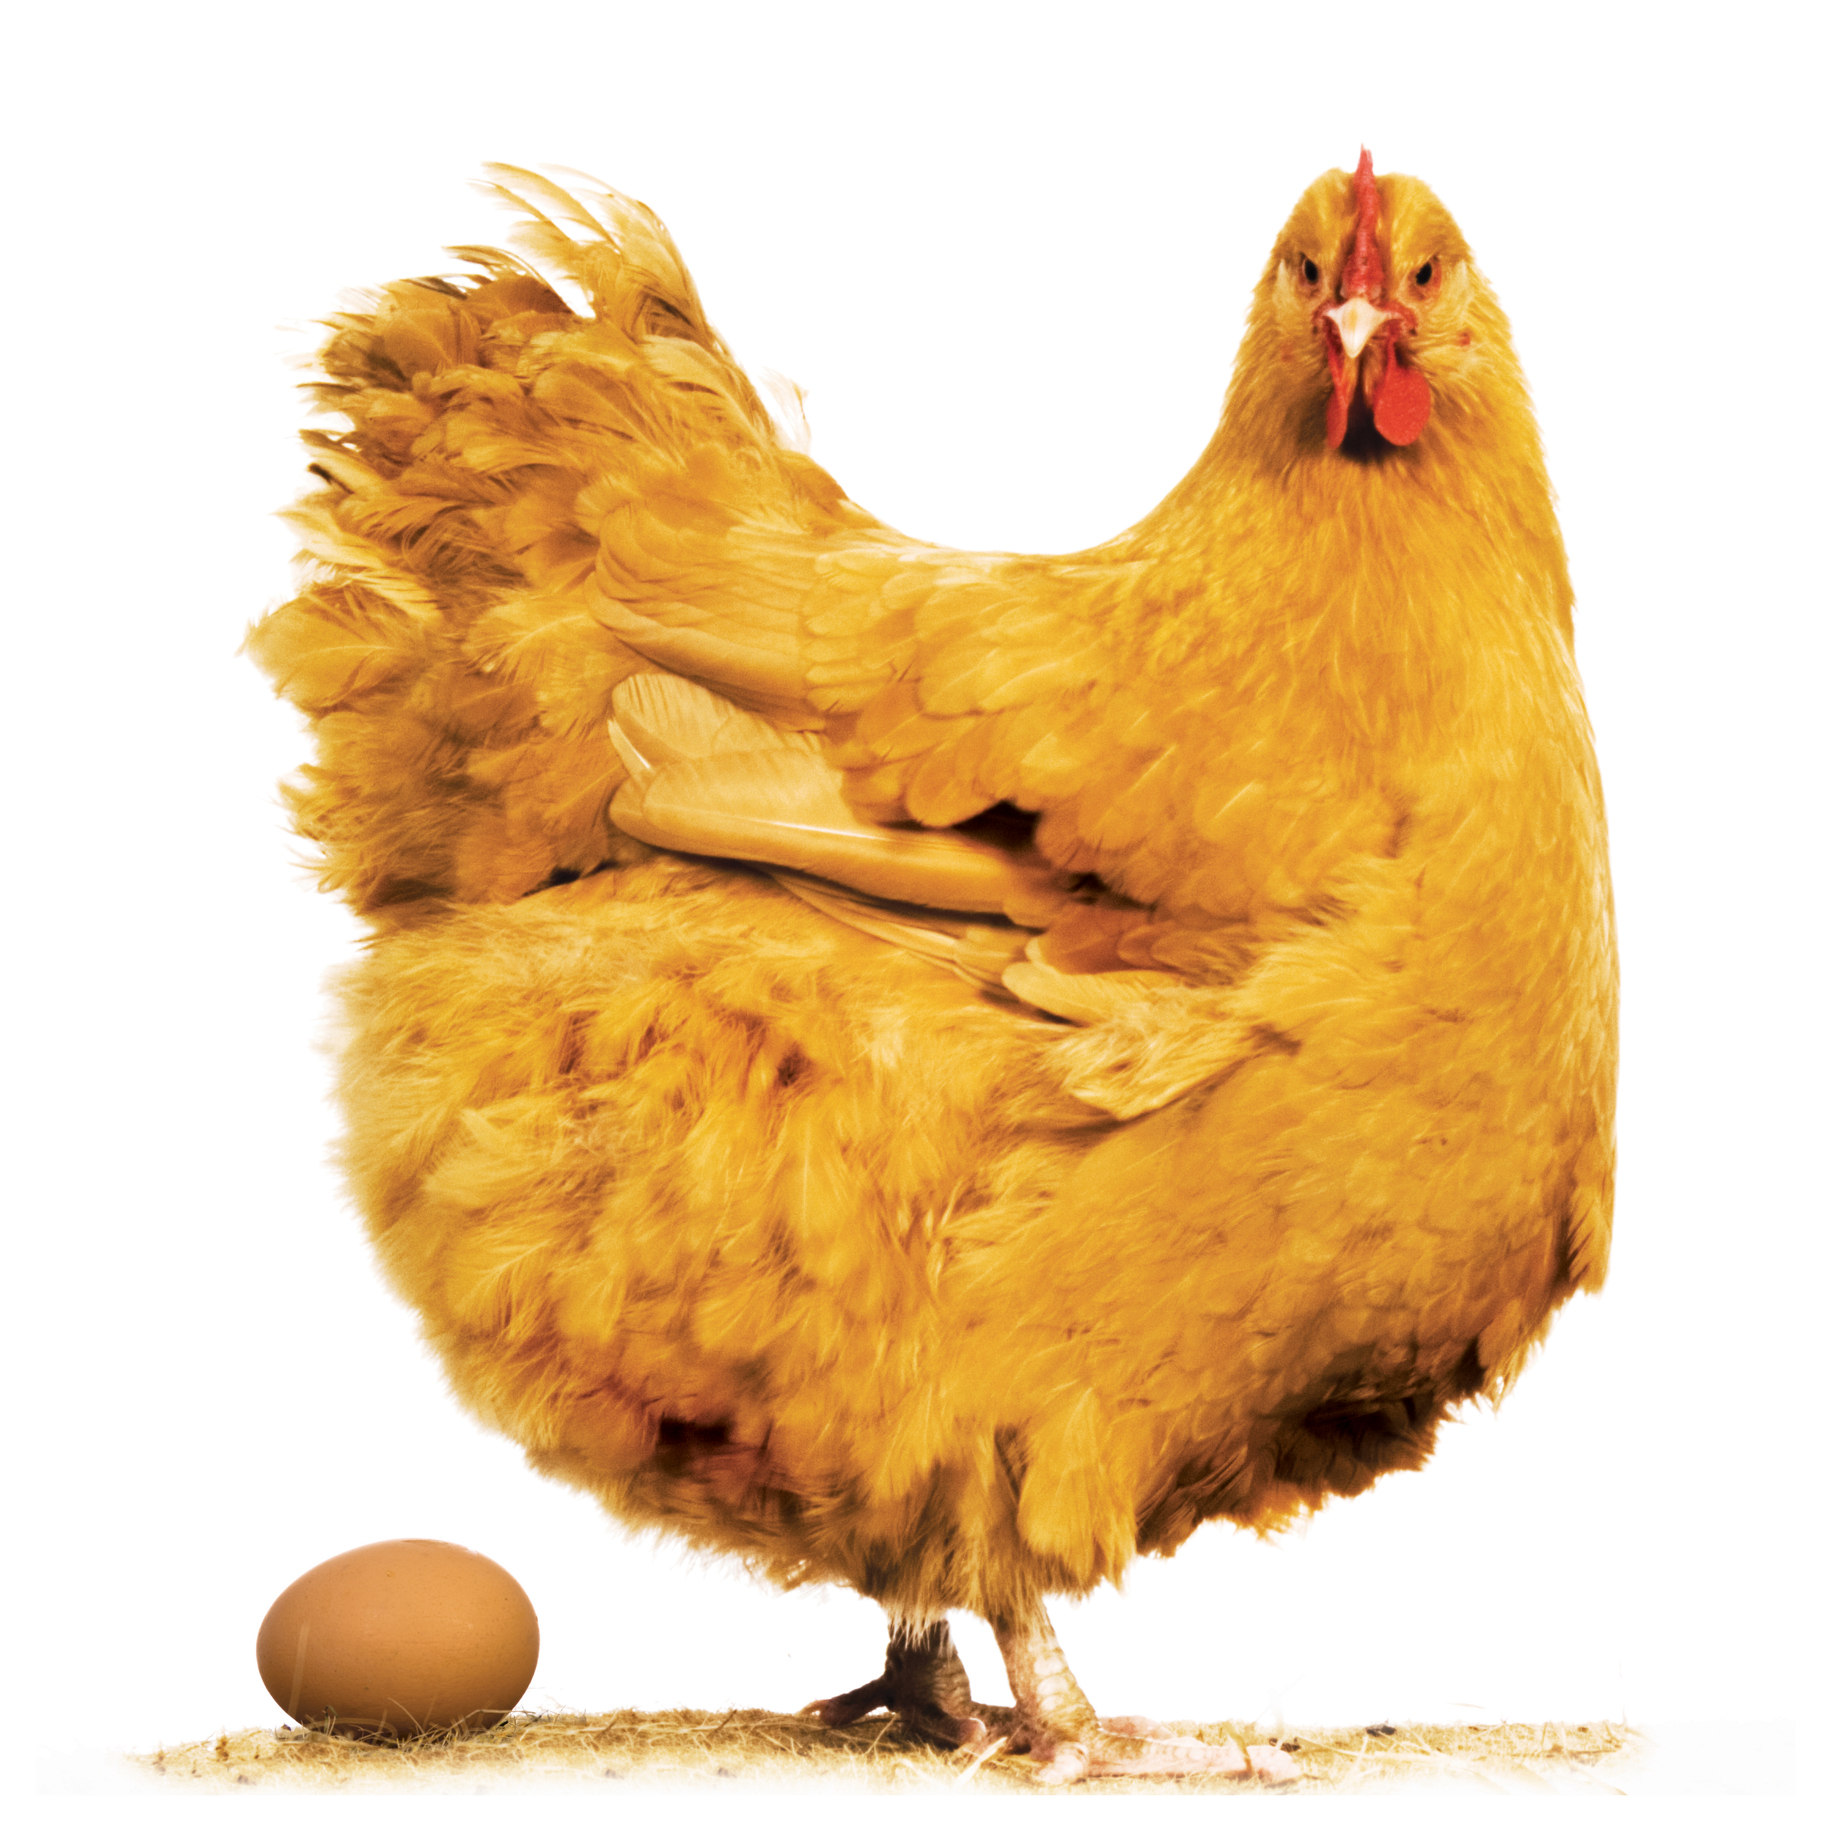
\includegraphics[width=0.80\textwidth]{chicken-and-egg.jpg}
                  \end{column}
                \end{columns}
              \end{block}

              \begin{block}{Direct estimation of $P$}
                \textbf{Alternative}: directly estimate $P$ from $X_{1:t}$.

                \smallskip
                \textbf{Key advantage}: observable confidence
                intervals for $P$ via ``empirical Bernstein''
                inequality for martingales.

                \smallskip
                \textbf{Two problems}:
                \begin{list}{$\triangleright$}\compresslist
                  \item
                    w/o using symmetry structure via $L$, can argue
                    \[
                      \norm{\wh{P} - P} \ \leq \ \veps
                      \ \Longrightarrow \
                      \abs{\hatgap - \gap} \ \leq \ O(\veps^{1/(2d)})
                      \,,
                    \]
                    but this implies \AWESOME{exponential slow-down in rate}.

                  \item
                    Using symmetry structure via $L$, get bounds that
                    depend on $\pi$, which is unknown.

                \end{list}

                \begin{center}
                  \BLUE{%
                    \textbf{Our approach}: \\
                    Directly estimate $P$, and \emph{indirectly} estimate $\pi$ via
                    $\wh P$.
                  }
                \end{center}


              \end{block}
            }
          \end{minipage}
        \end{beamercolorbox}
      \end{column}
      \begin{column}{0.24\textwidth}
        \begin{beamercolorbox}[center,wd=\textwidth]{postercolumn}
          \begin{minipage}[T]{.95\textwidth}
            \parbox[t][\columnheight]{\textwidth}{
              \begin{block}{Indirect estimation of $\pi$}

                \begin{list}{$\triangleright$}\compresslist
                  \item
                    Ensure that $\wh P$ is transition operator for
                    ergodic chain {\small(easy via Laplace
                    smoothing)}.

                    \smallskip

                  \item
                    Estimate $\pi$ via $\wh P$ via \GREEN{group
                    inverse} $\wh A^\#$ of $I - \wh P$.

                    \smallskip

                    \begin{itemize}\compresslist
                      \item
                        $\wh A^\#$ contains ``virtually everything
                        that one would want to know about the chain''
                        {\small(Meyer, 1975)}.

                        \smallskip

                      \item
                        Reveals unique stationary distribution $\hat\pi$ w.r.t.~$\wh P$.

                        \BLUE{This is our indirect estimate of $\pi$}.

                        \smallskip

                      \item
                        Gives
                        bound on $\norm{\hat\pi-\pi}_\infty$ in terms of
                        $\norm{\wh P - P}$.

                        \BLUE{With this, we construct a confidence interval
                        for $\pi$.}

                    \end{itemize}

                \end{list}

              \end{block}

%              \begin{block}{Overall algorithm (outline)}
%                \begin{list}{$\triangleright$}\compresslist
%                  \item
%                    Form empirical estimate and CI's for $P$
%
%                    {\small(exploit Markov property \& ``empirical Bernstein''-type bounds)}.
%
%                    \medskip
%
%                  \item
%                    Form estimate and CI's for $\pi$
%
%                    {\small(via group inverse of $I - \wh P$)}.
%
%                    \medskip
%
%                  \item
%                    Form estimate and CI's for $\gap$
%
%                    {\small(via CI's for $\pi$ and $P$, \& eigenvalue perturbation theory)}.
%
%                \end{list}
%
%              \end{block}
%
              \begin{block}{Overall algorithm}
                \begin{algorithmic}[1]
                  \STATE Compute state visit counts and smoothed transition
                  probability estimates:
                  \begin{equation}
                    \begin{aligned}
                      N_i & :=
                      \Abs{
                        \Braces{
                          \tau \in [t{-}1] : X_\tau = i
                        }
                      }
                      \,, \\
                      N_{i,j} & :=
                      \Abs{
                        \Braces{
                          \tau \in [t{-}1] : (X_\tau,X_{\tau+1}) = (i,j)
                        }
                      }
                      \,, \\
                      \wh{P}_{i,j}
                      & :=
                      \frac{N_{i,j} + 1/d}{N_i + 1}
                      \,.
                    \end{aligned}
                    \notag
                  \end{equation}

                  \STATE Let $\giAh$ be the group inverse of $\wh\vA := \vI -
                  \wh\vP$.

                  \STATE Let $\hat\vpi \in \Delta^{d-1}$ be stationary
                  distribution for $\wh\vP$.

                  \STATE Compute eigenvalues
                  $\braces{\hat\lambda_i}_{i\in[d]}$ of
                  $0.5(\wh\vL+\wh\vL^\t)$, where $\wh\vL
                  := \Diag(\hat\vpi)^{1/2} \wh\vP \Diag(\hat\vpi)^{-1/2}$.

                  \STATE Gap estimate:
                    $\hatgap := 1 - \max\braces{ \hat\lambda_2,
                    |\hat\lambda_d| }$.

                  \STATE Empirical bounds for $|\wh{P}_{i,j}{-}P_{i,j}|$ for $(i,j){\in}[d]^2$:
                  \begin{equation}
                    \wh{B}_{i,j}
                    :=
                    O\Parens{
                      \sqrt{\frac{\wh P_{i,j}\log\frac{d\log t}\delta}{N_i}}
                      + \frac{\log\frac{d\log t}\delta}{N_i}
                    }
                    .
                    \notag
                  \end{equation}

                  \STATE Relative sensitivity of $\vpi$:
                  \begin{equation}
                    \hat\kappa :=
                    \frac12
                    \max_{j\in[d]}
                    \Braces{
                      \wh{A}_{j,j}^\# - \min_{i\in[d]}\Braces{ \wh{A}_{i,j}^\# }
                    } 
                    .
                    \notag
                  \end{equation}

                  \STATE Empirical bounds for $\max_{i \in [d]} |\hat{\pi}_i -
                  \pi_i|$ and
                  $\max\bigcup_{i\in[d]}
                  \braces{
                    \abs{\sqrt{\pi_i/\hat\pi_i}-1},\,
                    \abs{\sqrt{\hat\pi_i/\pi_i}-1}
                  }$:
                  \begin{align*}
                    \hat{b}
                    & := \hat\kappa \max\Braces{
                      \wh{B}_{i,j}
                      : (i,j) \in [d]^2
                    }
                    , \\
                    \hat\rho
                    & := \frac12 \max \bigcup_{i\in[d]}
                    \Braces{
                      \frac{\hat{b}}{\hat\pi_i},\,
                      \frac{\hat{b}}{\brackets{\hat\pi_i-\hat{b}}_+}
                    }
                    .
                  \end{align*}

                  \STATE Empirical bounds for $\abs{\hatgap-\gap}$:
                  \begin{equation}
                    \hat{w} := 2\hat\rho + \hat\rho^2
                    + (1+2\hat\rho+\hat\rho^2)
                    \Biggl(
                      \sum_{(i,j)\in[d]^2} \frac{\hat\pi_i}{\hat\pi_j} \hat{B}_{i,j}^2
                    \Biggr)^{1/2} .
                    \notag
                  \end{equation}

                \end{algorithmic}
              \end{block}

            }
          \end{minipage}
        \end{beamercolorbox}
      \end{column}
    \end{columns}

    \vfill
  \end{frame}
\end{document}

